\documentclass[a4paper,12pt]{article}
\usepackage{tikz}
\usepackage[top=2cm,bottom=3cm,left=1.5cm,right=1.5cm]{geometry}
\usepackage[lined,algo2e,boxed]{algorithm2e}
\usepackage{listings}
\usepackage{amsmath}
\usepackage{hyperref}
\usepackage{url}
\usepackage{float}
\usepackage{subfigure}
\graphicspath{{img/}}

%%% CODE SNIPPETS, COMMANDS, ETC
%%%-----------------------------------------------------------------------------
\usepackage{xcolor}
\usepackage{listings} % Display code / shell commands
\usepackage{lstautogobble}
\usepackage{xspace}
\usepackage{xcolor}
\usepackage{listings} % Display code / shell commands
\usepackage{lstautogobble}
%\newcommand{\shellcommand}[1]{\begin{lstlisting} \#1 \end{lstlisting}
\lstdefinestyle{BashInputStyle}{
  language=bash,
  basicstyle=\small\ttfamily,
%  numbers=left,
%  numberstyle=\tiny,
%  numbersep=3pt,
  frame=single,
  columns=fullflexible,
  backgroundcolor=\color{yellow!10},
  linewidth=0.95\linewidth,
  xleftmargin=0.05\linewidth,
  keepspaces=true,
  framesep=5pt,
  rulecolor=\color{black!30},
  aboveskip=10pt,
  autogobble=true
}
\definecolor{gray}{rgb}{0.4,0.4,0.4}
\definecolor{darkblue}{rgb}{0.0,0.0,0.6}
\definecolor{darkred}{rgb}{0.6,0.0,0.0}
\definecolor{cyan}{rgb}{0.0,0.6,0.6}
\definecolor{maroon}{rgb}{0.5,0.0,0.0}
\lstdefinelanguage{XML}
{
  basicstyle=\ttfamily\footnotesize,
  morestring=[b]",
  moredelim=[s][\bfseries\color{maroon}]{<}{\ },
  moredelim=[s][\bfseries\color{maroon}]{</}{>},
  moredelim=[l][\bfseries\color{maroon}]{/>},
  moredelim=[l][\bfseries\color{maroon}]{>},
  morecomment=[s]{<?}{?>},
  morecomment=[s]{<!--}{-->},
  commentstyle=\color{gray},
  stringstyle=\color{orange},
  identifierstyle=\color{darkblue}
}
\lstdefinestyle{XMLStyle}{
  language=XML,
  basicstyle=\sffamily\footnotesize,
  numbers=left,
  numberstyle=\tiny,
  numbersep=3pt,
  frame=,
  columns=fullflexible,
  backgroundcolor=\color{black!05},
  linewidth=0.95\linewidth,
  xleftmargin=0.05\linewidth
}
\lstdefinestyle{C++Style}{
  language=C++,
  basicstyle=\sffamily\footnotesize,
  numbers=left,
  numberstyle=\tiny,
  numbersep=3pt,
  frame=,
  columns=fullflexible,
  backgroundcolor=\color{black!05},
  linewidth=0.9\linewidth,
  xleftmargin=0.1\linewidth,
  showspaces=false,
  showstringspaces=false
}


\usepackage{tikz}
\newcommand{\inltt}[1]{\tikz[anchor=base,baseline]\node[inner sep=3pt,
rounded corners,outer sep=0,draw=black!30,fill=black!05]{\small\texttt{#1}};}
\newcommand{\inlsh}[1]{\tikz[anchor=base,baseline]\node[inner sep=2pt,
outer sep=0,fill=black!05]{\texttt{#1}};}
\newcommand{\nekpp}{{\em Nektar++}\xspace}

% Highlight box
\usepackage{environ}
\usepackage[tikz]{bclogo}
\usetikzlibrary{calc}
\NewEnviron{notebox}
  {\par\medskip\noindent
  
\begin{tikzpicture}
    \node[inner sep=5pt,fill=black!10,draw=black!30] (box)
    {\parbox[t]{.99\linewidth}{%
      \begin{minipage}{.1\linewidth}
      \centering\tikz[scale=1]\node[scale=1.5]{\bcinfo};
      \end{minipage}%
      \begin{minipage}{.9\linewidth}
      \textbf{Note}\par\smallskip
      \BODY
      \end{minipage}\hfill}%
    };
   \end{tikzpicture}\par\medskip%
}
\NewEnviron{warningbox}
  {\par\medskip\noindent
  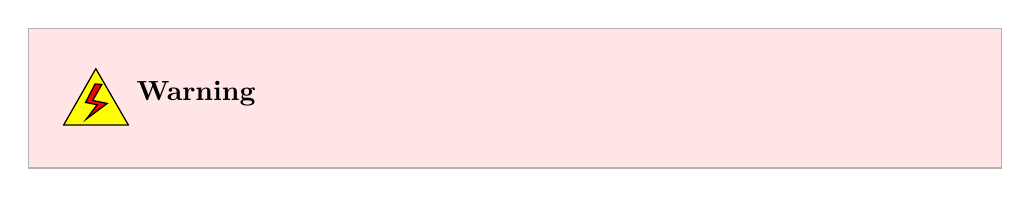
\begin{tikzpicture}
    \node[inner sep=5pt,fill=red!10,draw=black!30] (box)
    {\parbox[t]{.99\linewidth}{%
      \begin{minipage}{.1\linewidth}
      \centering\tikz[scale=1]\node[scale=1.5]{\bcdanger};
      \end{minipage}%
      \begin{minipage}{.9\linewidth}
      \textbf{Warning}\par\smallskip
      \BODY
      \end{minipage}\hfill}%
    };
   \end{tikzpicture}\par\medskip%
}
\NewEnviron{tipbox}
  {\par\medskip\noindent
  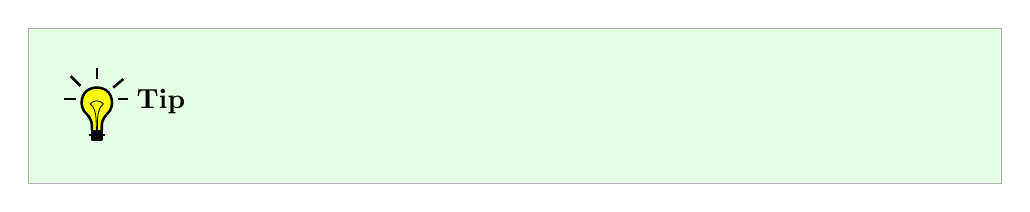
\begin{tikzpicture}
    \node[inner sep=5pt,fill=green!10,draw=black!30] (box)
    {\parbox[t]{.99\linewidth}{%
      \begin{minipage}{.1\linewidth}
      \centering\tikz[scale=1]\node[scale=1.5]{\bclampe};
      \end{minipage}%
      \begin{minipage}{.9\linewidth}
      \textbf{Tip}\par\smallskip
      \BODY
      \end{minipage}\hfill}%
    };
   \end{tikzpicture}\par\medskip%
}
\NewEnviron{custombox}[3]
  {\par\medskip\noindent
  \begin{tikzpicture}
    \node[inner sep=5pt,fill=#3!10,draw=black!30] (box)
    {\parbox[t]{.99\linewidth}{%
      \begin{minipage}{.1\linewidth}
      \centering\tikz[scale=1]\node[scale=1.5]{#2};
      \end{minipage}%
      \begin{minipage}{.9\linewidth}
      \textbf{#1}\par\smallskip
      \BODY
      \end{minipage}\hfill}%
    };
   \end{tikzpicture}\par\medskip%
}


\newcounter{taskcount}[section]
\newcommand\gmsh{\emph{Gmsh}~}
\newcommand\paraview{\emph{Paraview}}
\newcommand\nektar{\emph{Nektar++~}}
\newcommand\tutorialpath{\texttt{/nektutorial}}
\newcommand\tutorialtask[1]{
    \addtocounter{taskcount}{1}
    \begin{center}
        \setlength{\fboxsep}{10pt}
        \colorbox{LightGrey}{
            \parbox{0.95\linewidth}{\textbf{Task
            \arabic{section}.\arabic{taskcount}}\par #1}
            }
    \end{center}
}
\newcommand\tutorialcommand[1]{
    \par{\vspace{1ex}
         \addtolength{\leftskip}{2mm}\texttt{#1}\par\vspace{1ex}}
}
\newcommand\tutorialnote[1]{\par{\textbf{Note: }#1}}

\setlength{\parindent}{0pt}
\setlength{\parskip}{1ex} 
\definecolor{LightGrey}{rgb}{0.9,0.9,0.9}

\title{Global Instability Computations: \nektar Installation}
\author{Crete}
\date{24th September 2015}

\begin{document}
\maketitle

The \nektar website is: \url{http://www.nektar.info}. Here you can find all 
the information needed for compiling and using the library. You can also 
find additional information regarding the development team, the applications 
and other related aspects. 

In the following we report the steps required for downloading and installing
\nektar.

\section{Install prerequisites}
It is assumed the tutorial will be undertaken on a computer running either:
\begin{itemize}
\item \textbf{Linux} or
\item \textbf{Mac OSX}.
\end{itemize}

In order to configure and compile \nektar along with the third-party libraries 
used, such as the ARPACK library, you will need the following tools:
\begin{itemize}
\item \textbf{CMake} to configure \nektar. This can be downloaded from 
\href{http://www.cmake.org/download/}{\underline{CMake}}. A binary version 
suitable for your operating system is acceptable;
\item a \textbf{C++ compiler} (e.g. g++) to compile \nektar;
\item the third-party \textbf{ARPACK library} used for the stability analysis 
tutorial and specifically for the Implicitly Restarted Arnoldi Method. 
The source code can be downloaded from 
\href{http://www.caam.rice.edu/software/ARPACK/download.html#ARPACK}{
\underline{ARPACK}}, along with the compilation and installation instructions;
\item a \textbf{Fortran compiler} to compile the ARPACK library.
\item \textbf{Boost} $> 1.52$. However, if this is not installed on 
your system, \nektar will download and compile it for you;
\item \textbf{FFTW}. However, if this is not installed on 
your system, \nektar will download and compile it for you.
\end{itemize}

If the links provided above are broken, just search for CMake and ARPACK 
using a web search engine.



\section{Nektar++ Compilation}
In most cases, this should be straightforward. 
For details, see the
\href{http://www.nektar.info/downloads/18}{\underline{User-Guide}} 
available from the downloads section of the website.

\begin{enumerate}
	\item Download the \nektar .tar.gz file - release 4.2.0 - from
	\href{http://www.nektar.info/downloads}{\underline{nektar++}}.
	\item Unpack the archive:
	\begin{lstlisting}[style=BashInputStyle]
	tar -xvf nektar++-4.2.0.tar.gz
	\end{lstlisting}
	Note that some OS save the .tar.gz file as a .tar file. If this is the case you
	need use the same command as above but with the correct extension of the file
	you are unpacking:
	\begin{lstlisting}[style=BashInputStyle]
	tar -xvf nektar++-4.2.0.tar
	\end{lstlisting}
	\item Enter the \inlsh{nektar++-4.2.0} directory and create a build directory
	\begin{lstlisting}[style=BashInputStyle]
	cd nektar++-4.2.0
	mkdir build
	cd build
	\end{lstlisting}
	\item Configure the build using CMake
	\begin{lstlisting}[style=BashInputStyle]
	ccmake ../
	\end{lstlisting}
	Press 'c' to perform an initial configuration. Enable the options
	\inlsh{NEKTAR\_USE\_ARPACK} and \inlsh{NEKTAR\_USE\_FFTW}; 
	configure again by pressing 'c' twice. When complete, press 'g' to 
	generate the build files.
	\item Compile the code
	\begin{lstlisting}[style=BashInputStyle]
	make -jX install
	\end{lstlisting}
	Replace 'X' with the number of processor cores in your computer to compile 
	in parallel.
	\begin{notebox}
	During the first stages of the compilation process, the \nektar build system
	will download and compile a number of other third-party libraries, if it has
	been unable to find them on your system. Please be patient.
	\end{notebox}
	\item Test the code
	\begin{lstlisting}[style=BashInputStyle]
	ctest -jX
	\end{lstlisting}
	Replace 'X' with the number of processor cores in your computer to 
	run the tests in parallel. If all the tests pass, you are ready for the tutorial!
\end{enumerate}

\section{Problems?}
If you have difficulties in getting \nektar working, please feel free to contact
us:
\begin{itemize}
	\item Gianmarco Mengaldo (g.mengaldo11@imperial.ac.uk)
	\item Chris Cantwell (c.cantwell@imperial.ac.uk)
	\item Spencer Sherwin (s.sherwin@imperial.ac.uk)
\end{itemize}
Alternatively, we would be happy to help you in person during the summer school,
prior to the \nektar session.
\end{document}
